\documentclass{article}

\usepackage[table,xcdraw]{xcolor}
\usepackage{fancyhdr}
\usepackage{extramarks}
\usepackage{amsmath}
\usepackage{amsthm}
\usepackage{amsfonts}
\usepackage{tikz}
\usepackage[plain]{algorithm}
\usepackage{algpseudocode}
\usepackage{enumerate}

\usepackage{listings}
\usepackage{forest}
\usepackage[shortlabels]{enumitem}

\usepackage{pgfplots}
\usepgfplotslibrary{colorbrewer}


\setlist[enumerate, 1]{1\textsuperscript{o}}
\lstset { %
    language=C++,
        backgroundcolor=\color{black!5}, % set backgroundcolor
            basicstyle=\footnotesize,% basic font setting
}

%\usetikzlibrary{automata,positioning}
\usetikzlibrary{positioning,shapes,shadows,arrows,automata}

%
% Basic Document Settings
%

\topmargin=-0.45in
\evensidemargin=0in
\oddsidemargin=0in
\textwidth=6.5in
\textheight=9.0in
\headsep=0.25in

\linespread{1.1}

\pagestyle{fancy}
\lhead{\hmwkAuthorName}
\rhead{ (\hmwkClassInstructor\ \hmwkClassTime): \hmwkTitle}
\lfoot{\lastxmark}
\cfoot{\thepage}

\renewcommand\headrulewidth{0.4pt}
\renewcommand\footrulewidth{0.4pt}

\setlength\parindent{0pt}

%
% Create Problem Sections
%

\newcommand{\enterProblemHeader}[1]{
    \nobreak\extramarks{}{Problem \arabic{#1} continued on next page\ldots}\nobreak{}
    \nobreak\extramarks{Problem \arabic{#1} (continued)}{Problem \arabic{#1} continued on next page\ldots}\nobreak{}
}

\newcommand{\exitProblemHeader}[1]{
    \nobreak\extramarks{Problem \arabic{#1} (continued)}{Problem \arabic{#1} continued on next page\ldots}\nobreak{}
    \stepcounter{#1}
    \nobreak\extramarks{Problem \arabic{#1}}{}\nobreak{}
}

\setcounter{secnumdepth}{0}
\newcounter{partCounter}


\newcommand{\hmwkTitle}{Assignment \#2}
\newcommand{\hmwkDueDate}{May 4th, 2016}
\newcommand{\hmwkClass}{CS515 Parallel Programming}
\newcommand{\hmwkClassTime}{Spring 2016}
\newcommand{\hmwkClassInstructor}{Jingke Li}
\newcommand{\hmwkAuthorName}{Konstantin Macarenco}


\title{
    \vspace{2in}
    \textmd{\textbf{\hmwkClass:\ \hmwkTitle}}\\
        \normalsize\vspace{0.1in}\small{Due\ on\ \hmwkDueDate\ at 11:59pm}\\
        \vspace{0.1in}\large{\textit{\hmwkClassInstructor\ \hmwkClassTime}}
    \vspace{3in}
}

\author{\textbf{\hmwkAuthorName}}
\date{}

\renewcommand{\part}[1]{\textbf{\large Part \Alph{partCounter}}\stepcounter{partCounter}\\}

%
% Various Helper Commands
%

% Useful for algorithms
\newcommand{\alg}[1]{\textsc{\bfseries \footnotesize #1}}

% For derivatives
\newcommand{\deriv}[1]{\frac{\mathrm{d}}{\mathrm{d}x} (#1)}

% For partial derivatives
\newcommand{\pderiv}[2]{\frac{\partial}{\partial #1} (#2)}

% Integral dx
\newcommand{\dx}{\mathrm{d}x}

% Alias for the Solution section header
\newcommand{\solution}{\textbf{\large Solution}}

% Probability commands: Expectation, Variance, Covariance, Bias
\newcommand{\E}{\mathrm{E}}
\newcommand{\Var}{\mathrm{Var}}
\newcommand{\Cov}{\mathrm{Cov}}
\newcommand{\Bias}{\mathrm{Bias}}

\begin{document}
\maketitle

\pagebreak

\section{\textbf{Primes}}
As you can see from the graph - parallel Primes algorithm performed better than sequential
version in all cases, with
one exception: OMP with one thread is always slower than the sequential implementation. 
This can be explained by overhead that is introduced by using OMP.

There are two possible solutions to the homework
\begin{enumerate}[1.]
\item Each thread works independently and starts crossing out multiples as fast as it finds a
non zero entry. The main disadvantage of this approach is that, since there is no
synchronization some thread will perform redundant jobs, and cross out some entries multiple
times.
\item Implement synchronization to avoid redundant job. In this case we need set of explicit
locks, waits, array partitioning, and a way to notify other threads about index being crossed out.
This most likely will result in worse performance than the first case.
\end{enumerate}

I used the first solution, and you can observe that increasing number of threads gives small
performance boost, with 128 being the fastest.\\

\begin{centering}
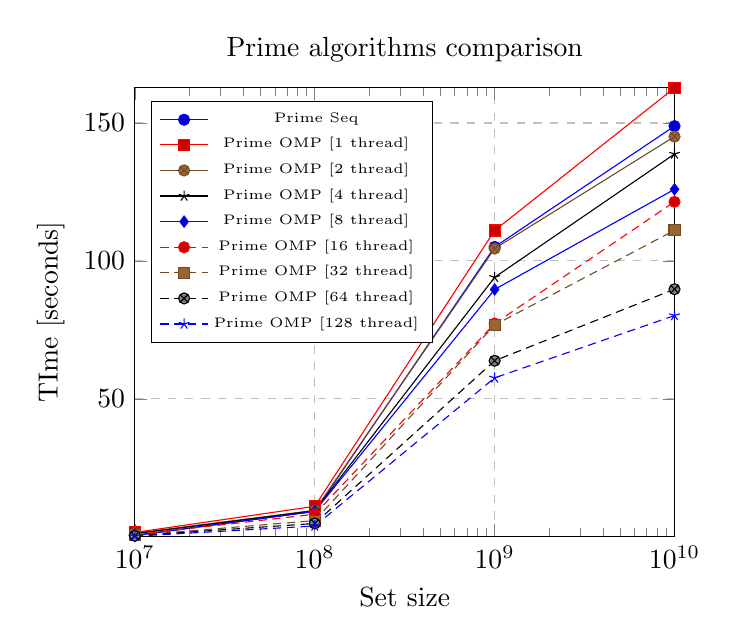
\begin{tikzpicture}
\begin{semilogxaxis}[
title={Prime algorithms comparison},
xlabel={Set size},
ylabel={TIme [seconds]},
ymajorgrids=true,
xmajorgrids=true,
grid style=dashed,
enlargelimits=false,
scaled y ticks=false,
xticklabel style={
        /pgf/number format/.cd,
        sci,
        sci generic={mantissa sep=\times,exponent={10^{#1}}}
},
legend style={legend pos=north west, font=\fontsize{4}{5}\selectfont},
]

\addplot coordinates { (10^7,0.533)(10^8, 9.161)(10^9, 105.080)(10^10, 148.891) }; \addlegendentry{Prime Seq}
\addplot coordinates { (10^7,1.548) (10^8,11.032)(10^9, 111.028)(10^10,162.742) }; \addlegendentry{Prime OMP [1 thread]} 
\addplot coordinates { (10^7, 1.268) (10^8, 9.572) (10^9, 104.474) (10^10, 145.092) }; \addlegendentry{Prime OMP [2 thread]}
\addplot coordinates { (10^7,1.097)(10^8,9.413)(10^9,94.059)(10^10,138.766) }; \addlegendentry{Prime OMP [4 thread]}
\addplot coordinates { (10^7,0.400)(10^8,9.203)(10^9,89.660)(10^10,125.969) }; \addlegendentry{Prime OMP [8 thread]}
\addplot coordinates { (10^7,0.753)(10^8,8.149)(10^9,77.292)(10^10,121.433) }; \addlegendentry{Prime OMP [16 thread]}
\addplot coordinates { (10^7,0.478) (10^8,5.845) (10^9,76.765) (10^10,111.086) }; \addlegendentry{Prime OMP [32 thread]}
\addplot coordinates { (10^7,0.337) (10^8,4.807) (10^9,63.811) (10^10,89.739) }; \addlegendentry{Prime OMP [64 thread]}
\addplot coordinates { (10^7,0.192) (10^8,3.904) (10^9,57.598) (10^10,80.190) }; \addlegendentry{Prime OMP [128 thread]}
\end{semilogxaxis}
\end{tikzpicture}
\end{centering}



\begin{table}[h!]
\begin{minipage}{0.48\textwidth}
\centering
\caption{Sequential execution (Time [sec])}
\label{my-label}
\begin{tabular}{lllll}
&      $10^7$           &    $10^8$    & $10^9$ &  $10^{10}$    \\ \hline
prime          &     0.533           &   9.616  & 105.080  & 148.891  \\ \hline
quicksort      &     4.247          &    39.907 & 425.748  & 653.039 \\
\end{tabular}
\end{minipage}%
\begin{minipage}{0.48\textwidth}
\centering
\caption{Prime omp (Time [sec])}
\label{my-label}
\begin{tabular}{l|llll}
&      $10^7$                             &    $10^8$    & $10^9$    &  $10^{10}$    \\ \hline
1       &       1.548                     &   11.032  & 111.028 & 162.742     \\ \hline
2       &       1.268                     &   9.572   & 104.474 & 145.092     \\ \hline
4       &       1.097                     &   9.413   & 94.059 &  138.766     \\ \hline
8       &       0.400                     &   9.203   & 89.660 &  125.969      \\ \hline
16       &      0.753                     &   8.149   & 77.292 &  121.433      \\ \hline
32       &      0.478                     &   5.845   & 76.765 &  111.086     \\ \hline
64       &      0.337                     &   4.807   & 63.811  & 89.739     \\ \hline
128       & \cellcolor[HTML]{34FF34}    0.192        & \cellcolor[HTML]{34FF34}  3.904   & \cellcolor[HTML]{34FF34} 57.598 & \cellcolor[HTML]{34FF34} 80.190     \\ 
\end{tabular}
\end{minipage}%
\end{table}

\pagebreak

\section{\textbf{Quick sort}}

Quick sort is much more suitable for parallelization since we only need to wait for the
current chunk of the array to be partitioned and no other synchronization. At first I had
trouble with placing OMP statements in the correct place. When pragma's are added to the
quickSort routine, every time the method called new parallel region is declared, which
creates exponential of number of threads, and leads to poor performance. \\

After some research I used ``\# pragma omp task firstprivate(array, low, high)'' to declare a
region that should be executed by a separate thread thread, and firstprivate indicates that 
array, low and high must be initialized before entering parallel region. In this case an
existing thread is assigned new parallel region. \\

This approach nearly doubles the performance as soon as number of threads is two or more.
Further increase of threads, gives slower performance boost, about \%20 percent with each
level (up to 16 threads). After number of threads reached 32 we can see some performance
degradation by \%8 in average (with each thread number increase). 
This behaviour usually rises when number of threads exceeds number of available work,
managing these waiting threads creates additional penalty. Hence the slow down. And in 
this case threads have to wait for partitioning to be complete, and new values for low and
high to be computed. According to my test run most optimal number of cores for qsort is 16.

Another thing worth mentioning, one thread OMP quicksort struggles from the same issue as 
prime, it is slower than sequential version by a constant factor.

\subsection{\textbf{qsort-pthd}}

Pthread version of qsort is faster than sequential, but ($\approx 2x$ in the best case) slower 
than OMP. This is expected, since qsort-pthd has multiple bottlenecks, such as shared number
of producing methods, and queue. This version's performance peak is at NUMTHREADS=8, as
number of threads increased performance drops to sequential level or much worse. 
In all tests, except $10^9$, Pthread 32 threads performed the worst. I expected to see Pthd
128 being the slowest in all cases.  This discrepancy, could be related to Babbage
being a shared machine, with variable load.

\subsection{\textbf{PTHD vs OMP revisited}}

I decided to re-test quicksort to see if Pthread performance inconsistency is a  
result of public machine variable load, except this time I excluded array initialization
from time measurement, since it can take up to \%40 of total time. One complication I had
is granularity of such a test, standard clock() function is useless since it gives a total
CPU cycles of all participated cores, and C time library maximum granularity is 1 second.
I omitted tests for world sizes $10^7$ and less, since they were slower than 1 sec, and world
size $10^{10}$, since machine was too busy at the time.

OMP quicksort is about 3x time faster than the application with array init accounted for, 
where doubling threads gave about the same performance increase, with most optimal  number of threads =
16.\\
On the other hand, Pthread quicksort had similar performance, with one exception: slowest
case ``threads = 16'', not 32 as in the original run.  Performance decline was again
sporadic, with ``threads = 128'' being faster, than the worse case. 

\subsection{\textbf{Other issues}} 
When number of threads is greater than number of available cores, there most likely be
slowdown, unless some cores are waiting and can run additional threads.\\

\textbf{Results continued on the next page$\dots$}

\pagebreak

\textbf{Quicksort OMP vs Pthread (Array init time included)}\\

\begin{table}[h!]
\begin{minipage}{0.48\textwidth}
\centering
\caption{Quick Sort omp (Time [sec])}
\label{my-label}
\begin{tabular}{l|llll}
&      $10^7$           &    $10^8$ & $10^9$    &  $10^{10}$    \\ \hline
1       &       4.313   &   40.367  & 441.530 & 689.361    \\ \hline
2       &       2.336   &   24.254  & 265.905& 393.473    \\ \hline
4       &       1.603   &   16.793  & 180.163 & 270.030    \\ \hline
8       & \cellcolor[HTML]{34FF34}      1.359   & \cellcolor[HTML]{34FF34}  14.699  & 152.552 & 230.375    \\ \hline
16      &       1.710   &   14.954  & \cellcolor[HTML]{34FF34}130.645 & \cellcolor[HTML]{34FF34}197.896    \\ \hline
32      &       1.527   &   15.191  & 139.620 & 215.855    \\ \hline
64      &       1.965   &   20.295  & 148.494 & 231.565    \\ \hline
128     &       2.531   &   16.134  & 167.827 & 245.310    \\ 
\end{tabular}
\end{minipage}%
\begin{minipage}{0.48\textwidth}
\centering
\caption{Quick Sort pthread (Time [sec])}
\label{my-label}
\begin{tabular}{l|llll}
&      $10^7$       &    $10^8$    & $10^9$      &  $10^{10}$  \\ \hline
1       &       3.825     &   45.857  & 469.146  &  668.053    \\ \hline
2       &       2.820     &   32.870  & 364.625  &  485.091    \\ \hline
4       &       2.897     &   28.845  & 303.976  &  449.671    \\ \hline
8       &  \cellcolor[HTML]{34FF34}     2.796     &  \cellcolor[HTML]{34FF34} 30.014  & \cellcolor[HTML]{34FF34} 287.594  & \cellcolor[HTML]{34FF34} 446.297    \\ \hline
16      &       8.892     &   37.327  & 361.015  &  753.872    \\ \hline
32      &       18.957    &   207.082 & 976.707  &  1141.691   \\ \hline
64      &       17.203    &   178.471 & 881.260  &  826.079    \\ \hline
128     &       10.841    &   49.304  & 1033.700 &  738.495    \\ 
\end{tabular}
\end{minipage}%
\end{table}

\vspace{0.4cm}

\begin{minipage}{0.48\textwidth}
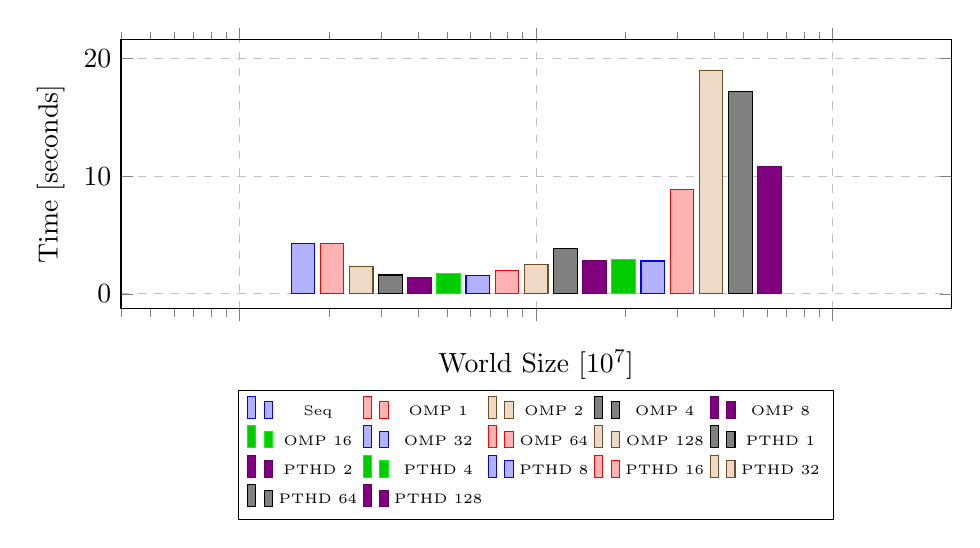
\begin{tikzpicture}
\begin{semilogxaxis}
%\begin{loglogaxis}
[ x tick label style={
    /pgf/number format/1000 sep=},
ylabel={Time [seconds]},
xlabel={World Size [$10^7$]},
legend style={at={(0.5,-0.3)},
    anchor=north,legend columns=5,font=\fontsize{3}{1}\selectfont},
ybar,
ymajorgrids=true,
xmajorgrids=true,
grid style=dashed,
enlargelimits=0.15,
scaled y ticks=false,
xticklabels= {,,},
height=5cm, width=\textwidth,
        bar width=0.3cm,
        ]
    \addplot coordinates {(10^7,4.247) }; 
    \addplot coordinates {(10^7,4.313) };
    \addplot coordinates {(10^7,2.336) };
    \addplot coordinates {(10^7,1.603) };
    \addplot coordinates {(10^7,1.359) };
    \addplot coordinates {(10^7,1.710) };
    \addplot coordinates {(10^7,1.527) };
    \addplot coordinates {(10^7,1.965) };
    \addplot coordinates {(10^7,2.531) };
    \addplot coordinates {(10^7,3.825) };
    \addplot coordinates {(10^7,2.820) };
    \addplot coordinates {(10^7,2.897) };
    \addplot coordinates {(10^7,2.796) };
    \addplot coordinates {(10^7,8.892) };
    \addplot coordinates {(10^7,18.957)};
    \addplot coordinates {(10^7,17.203)};
    \addplot coordinates {(10^7,10.841)};
\legend{Seq
, OMP 1 , OMP 2 , OMP 4 , OMP 8 , OMP 16 , OMP 32 , OMP 64 , OMP 128 , PTHD 1 , PTHD 2 , PTHD 4 , PTHD 8 , PTHD 16 , PTHD 32 , PTHD 64 , PTHD 128
}
%\end{loglogaxis}
\end{semilogxaxis}
\end{tikzpicture}
\end{minipage}%
\begin{minipage}{0.48\textwidth}
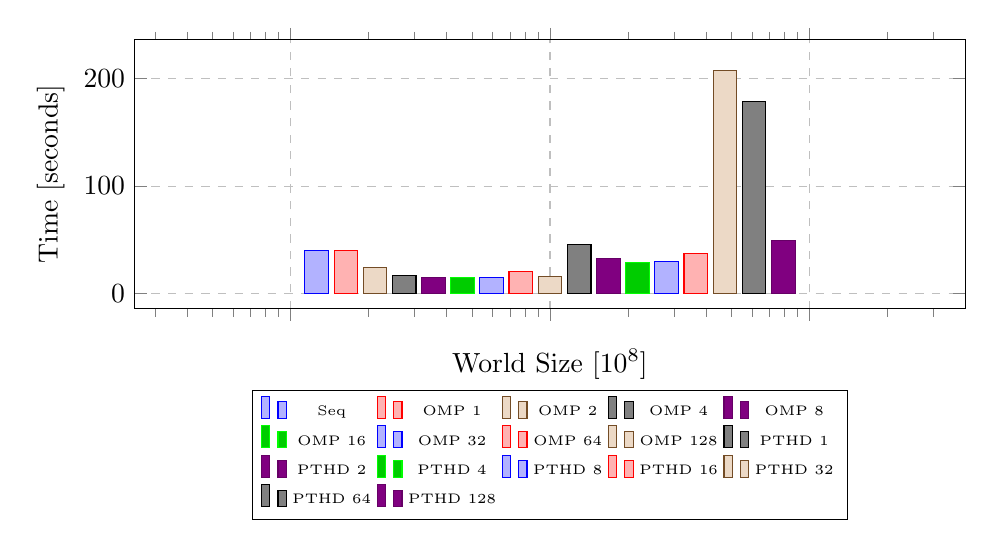
\begin{tikzpicture}
\begin{semilogxaxis}
%\begin{loglogaxis}
[ x tick label style={
    /pgf/number format/1000 sep=},
ylabel={Time [seconds]},
legend style={at={(0.5,-0.3)},
    anchor=north,legend columns=5,font=\fontsize{3}{1}\selectfont},
ybar,
ymajorgrids=true,
xmajorgrids=true,
xlabel={World Size [$10^8$]},
grid style=dashed,
enlargelimits=0.15,
scaled y ticks=false,
xticklabels= {,,},
height=5cm, width=\textwidth,
        bar width=0.3cm,
        ]
    \addplot coordinates {(10^8,39.907) }; 
    \addplot coordinates {(10^8,40.367) };
    \addplot coordinates {(10^8,24.254) };
    \addplot coordinates {(10^8,16.793) };
    \addplot coordinates {(10^8,14.699) };
    \addplot coordinates {(10^8,14.954) };
    \addplot coordinates {(10^8,15.191) };
    \addplot coordinates {(10^8,20.295) };
    \addplot coordinates {(10^8,16.134) };
    \addplot coordinates {(10^8,45.857) };
    \addplot coordinates {(10^8,32.870) };
    \addplot coordinates {(10^8,28.845) };
    \addplot coordinates {(10^8,30.014) };
    \addplot coordinates {(10^8,37.327) };
    \addplot coordinates {(10^8,207.082)};
    \addplot coordinates {(10^8,178.471)};
    \addplot coordinates {(10^8,49.304) };
\legend{Seq
, OMP 1 , OMP 2 , OMP 4 , OMP 8 , OMP 16 , OMP 32 , OMP 64 , OMP 128 , PTHD 1 , PTHD 2 , PTHD 4 , PTHD 8 , PTHD 16 , PTHD 32 , PTHD 64 , PTHD 128
}
%\end{loglogaxis}
\end{semilogxaxis}
\end{tikzpicture}
\end{minipage}%

\begin{minipage}{0.48\textwidth}
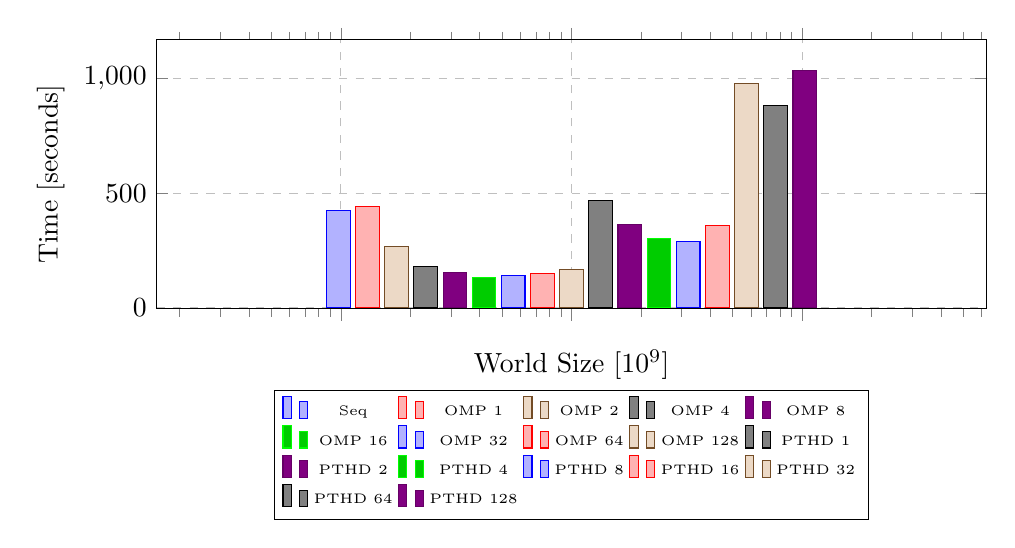
\begin{tikzpicture}
\begin{semilogxaxis}
%\begin{loglogaxis}
[ x tick label style={
    /pgf/number format/1000 sep=},
ylabel={Time [seconds]},
legend style={at={(0.5,-0.3)},
    anchor=north,legend columns=5,font=\fontsize{3}{1}\selectfont},
ybar,
ymajorgrids=true,
xmajorgrids=true,
grid style=dashed,
xlabel={World Size [$10^9$]},
enlargelimits=0.15,
xticklabels= {,,},
scaled y ticks=false,
height=5cm, width=\textwidth,
        bar width=0.3cm,
        ]
    \addplot coordinates {(10^9,425.748) }; 
    \addplot coordinates {(10^9,441.530) };
    \addplot coordinates {(10^9,265.905) };
    \addplot coordinates {(10^9,180.163) };
    \addplot coordinates {(10^9,152.552) };
    \addplot coordinates {(10^9,130.645) };
    \addplot coordinates {(10^9,139.620) };
    \addplot coordinates {(10^9,148.494) };
    \addplot coordinates {(10^9,167.827) };
    \addplot coordinates {(10^9,469.146) };
    \addplot coordinates {(10^9,364.625) };
    \addplot coordinates {(10^9,303.976) };
    \addplot coordinates {(10^9,287.594) };
    \addplot coordinates {(10^9,361.015) };
    \addplot coordinates {(10^9,976.707) };
    \addplot coordinates {(10^9,881.260) };
    \addplot coordinates {(10^9,1033.700)};
\legend{Seq
, OMP 1 , OMP 2 , OMP 4 , OMP 8 , OMP 16 , OMP 32 , OMP 64 , OMP 128 , PTHD 1 , PTHD 2 , PTHD 4 , PTHD 8 , PTHD 16 , PTHD 32 , PTHD 64 , PTHD 128
}
%\end{loglogaxis}
\end{semilogxaxis}
\end{tikzpicture}
\end{minipage}%
\begin{minipage}{0.48\textwidth}
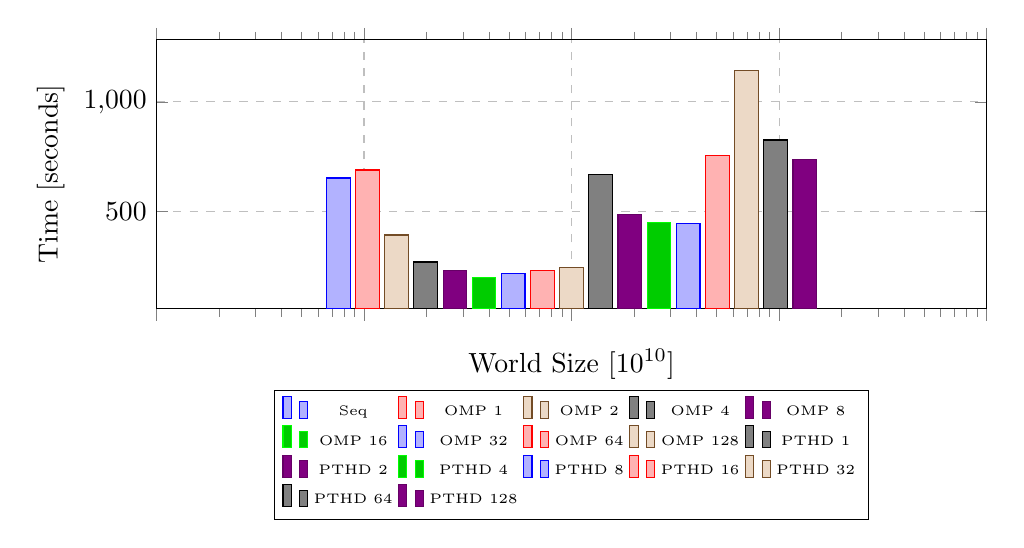
\begin{tikzpicture}
\begin{semilogxaxis}
%\begin{loglogaxis}
[ x tick label style={
    /pgf/number format/1000 sep=},
ylabel={Time [seconds]},
legend style={at={(0.5,-0.3)},
    anchor=north,legend columns=5,font=\fontsize{3}{1}\selectfont},
ybar,
ymajorgrids=true,
xmajorgrids=true,
grid style=dashed,
xlabel={World Size [$10^{10}$]},
enlargelimits=0.15,
scaled y ticks=false,
xticklabels= {,,},
height=5cm, width=\textwidth,
        bar width=0.3cm,
        ]
    \addplot coordinates {(10^10,653.039)}; 
    \addplot coordinates {(10^10,689.361)};
    \addplot coordinates {(10^10,393.473)};
    \addplot coordinates {(10^10,270.030)};
    \addplot coordinates {(10^10,230.375)};
    \addplot coordinates {(10^10,197.896)};
    \addplot coordinates {(10^10,215.855)};
    \addplot coordinates {(10^10,231.565)};
    \addplot coordinates {(10^10,245.310)};
    \addplot coordinates {(10^10,668.053)};
    \addplot coordinates {(10^10,485.091)};
    \addplot coordinates {(10^10,449.671)};
    \addplot coordinates {(10^10,446.297)};
    \addplot coordinates {(10^10,753.872)};
    \addplot coordinates {(10^10,1141.691)};
    \addplot coordinates {(10^10,826.079)};
    \addplot coordinates {(10^10,738.495)};
            %node[above] at (axis cs:10^10,500) {Houses};
\legend{Seq
, OMP 1 , OMP 2 , OMP 4 , OMP 8 , OMP 16 , OMP 32 , OMP 64 , OMP 128 , PTHD 1 , PTHD 2 , PTHD 4 , PTHD 8 , PTHD 16 , PTHD 32 , PTHD 64 , PTHD 128
}
%\end{loglogaxis}
\end{semilogxaxis}
\end{tikzpicture}
\end{minipage}

%\begin{tikzpicture}
%\begin{semilogxaxis}
%%\begin{loglogaxis}
%[ x tick label style={
%    /pgf/number format/1000 sep=},
%ylabel={Time [seconds]},
%legend style={at={(0.5,-0.1)},
%    anchor=north,legend columns=9,font=\fontsize{3}{1}\selectfont},
%ybar,
%ymajorgrids=true,
%xmajorgrids=true,
%grid style=dashed,
%enlargelimits=0.15,
%scaled y ticks=false,
%height=5cm, width=0.48\textwidth,
%        bar width=0.15cm,
%        ]
%    \addplot coordinates {(10^7,4.247) (10^8,39.907) (10^9,425.748) (10^10,653.039)}; 
%    \addplot coordinates {(10^7,4.313) (10^8,40.367) (10^9,441.530) (10^10,689.361)};
%    \addplot coordinates {(10^7,2.336) (10^8,24.254) (10^9,265.905) (10^10,393.473)};
%    \addplot coordinates {(10^7,1.603) (10^8,16.793) (10^9,180.163) (10^10,270.030)};
%    \addplot coordinates {(10^7,1.359) (10^8,14.699) (10^9,152.552) (10^10,230.375)};
%    \addplot coordinates {(10^7,1.710) (10^8,14.954) (10^9,130.645) (10^10,197.896)};
%    \addplot coordinates {(10^7,1.527) (10^8,15.191) (10^9,139.620) (10^10,215.855)};
%    \addplot coordinates {(10^7,1.965) (10^8,20.295) (10^9,148.494) (10^10,231.565)};
%    \addplot coordinates {(10^7,2.531) (10^8,16.134) (10^9,167.827) (10^10,245.310)};
%    \addplot coordinates {(10^7,3.825) (10^8,45.857) (10^9,469.146) (10^10,668.053)};
%    \addplot coordinates {(10^7,2.820) (10^8,32.870) (10^9,364.625) (10^10,485.091)};
%    \addplot coordinates {(10^7,2.897) (10^8,28.845) (10^9,303.976) (10^10,449.671)};
%    \addplot coordinates {(10^7,2.796) (10^8,30.014) (10^9,287.594) (10^10,446.297)};
%    \addplot coordinates {(10^7,8.892) (10^8,37.327) (10^9,361.015) (10^10,753.872)};
%    \addplot coordinates {(10^7,18.957)(10^*,207.082)(10^9,976.707) (10^10,1141.691)};
%    \addplot coordinates {(10^7,17.203)(10^*,178.471)(10^9,881.260) (10^10,826.079)};
%    \addplot coordinates {(10^7,10.841)(10^*,49.304) (10^9,1033.700)(10^10,738.495)};
%\legend{Seq)
%, OMP 1 , OMP 2 , OMP 4 , OMP 8 , OMP 16 , OMP 32 , OMP 64 , OMP 128 , PTHD 1 , PTHD 2 , PTHD 4 , PTHD 8 , PTHD 16 , PTHD 32 , PTHD 64 , PTHD 128
%}
%%\end{loglogaxis}
%\end{semilogxaxis}
%\end{tikzpicture}

\pagebreak

\textbf{Quicksort OMP vs Pthread (Array init time is not included)}\\

\begin{table}[h!]
\begin{minipage}{0.48\textwidth}
\centering
\caption{Quick Sort OMP (no init) (Time [sec])}
\label{my-label}
\begin{tabular}{l|ll}
&      $10^8$           &    $10^9$ \\ \hline
1       &       32   &   371        \\ \hline
2       &       16   &   188        \\ \hline
4       &       10   &   99         \\ \hline
8       &       5   &   61         \\ \hline
16      &       5   &   42           \\ \hline
32      &       6   &   52         \\ \hline
64      &       7   &   60         \\ \hline
128     &       10   &   80         \\ 
\end{tabular}
\end{minipage}%
\begin{minipage}{0.48\textwidth}
\centering
\caption{Quick Sort Pthread (no init)(Time [sec])}
\label{my-label}
\begin{tabular}{l|llll}
&      $10^8$       &    $10^9$       \\ \hline
1       &       36    &   408 \\ \hline
2       &       27    &   264 \\ \hline
4       &       22    &   231 \\ \hline
8       &       22    &   224     \\ \hline
16      &       33    &   348 \\ \hline
32      &       58    &   920 \\ \hline
64      &       51    &   582 \\ \hline
128     &       44    &   548 \\ 
\end{tabular}
\end{minipage}%
\end{table}




\begin{minipage}{0.48\textwidth}
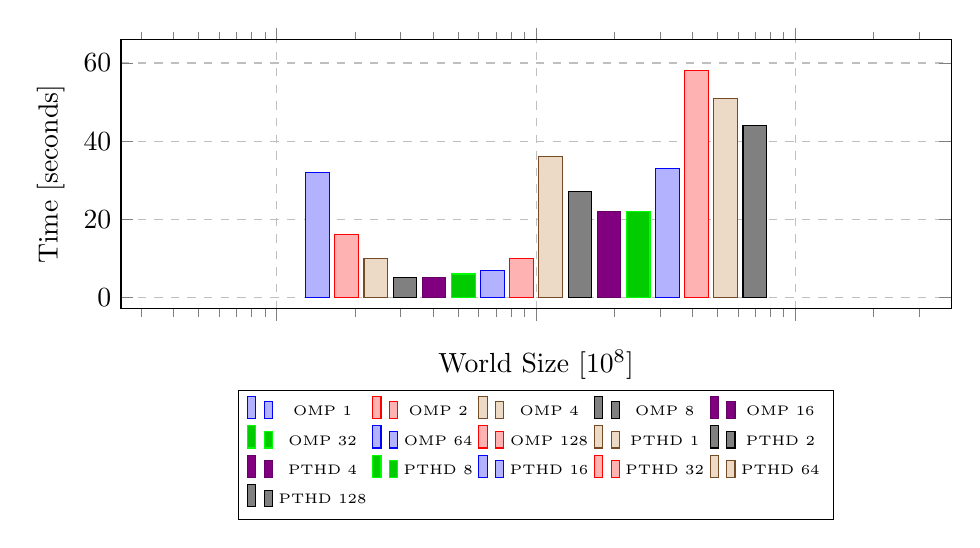
\begin{tikzpicture}
\begin{semilogxaxis}
%\begin{loglogaxis}
[ x tick label style={
    /pgf/number format/1000 sep=},
ylabel={Time [seconds]},
xlabel={World Size [$10^8$]},
legend style={at={(0.5,-0.3)},
    anchor=north,legend columns=5,font=\fontsize{3}{1}\selectfont},
ybar,
ymajorgrids=true,
xmajorgrids=true,
grid style=dashed,
enlargelimits=0.15,
scaled y ticks=false,
xticklabels= {,,},
height=5cm, width=\textwidth,
        bar width=0.3cm,
        ]
    \addplot coordinates {(10^8,32) }; 
    \addplot coordinates {(10^8,16) };
    \addplot coordinates {(10^8,10) };
    \addplot coordinates {(10^8,5) };
    \addplot coordinates {(10^8,5) };
    \addplot coordinates {(10^8,6) };
    \addplot coordinates {(10^8,7) };
    \addplot coordinates {(10^8,10) };
    \addplot coordinates {(10^8,36) }; 
    \addplot coordinates {(10^8,27) };
    \addplot coordinates {(10^8,22) };
    \addplot coordinates {(10^8,22) };
    \addplot coordinates {(10^8,33) };
    \addplot coordinates {(10^8,58) };
    \addplot coordinates {(10^8,51) };
    \addplot coordinates {(10^8,44) };
\legend{
OMP 1 , OMP 2 , OMP 4 , OMP 8 , OMP 16 , OMP 32 , OMP 64 , OMP 128 , PTHD 1 , PTHD 2 , PTHD 4 , PTHD 8 , PTHD 16 , PTHD 32 , PTHD 64 , PTHD 128
}
%\end{loglogaxis}
\end{semilogxaxis}
\end{tikzpicture}
\end{minipage}%
\begin{minipage}{0.48\textwidth}
\begin{tikzpicture}
\begin{semilogxaxis}
%\begin{axis}
%\begin{loglogaxis}
[ 
    % colorbrewer values=18,
    colorbrewer cycle list=Oranges,
    %cycle list name=Dark2,
    x tick label style={
    /pgf/number format/1000 sep=},
ylabel={Time [seconds]},
legend style={at={(0.5,-0.3)},
    anchor=north,legend columns=5,font=\fontsize{3}{1}\selectfont},
ybar,
ymajorgrids=true,
xmajorgrids=true,
xlabel={World Size [$10^9$]},
grid style=dashed,
enlargelimits=0.15,
scaled y ticks=false,
xticklabels= {,,},
height=5cm, width=\textwidth,
        bar width=0.3cm,
        ]
    \addplot coordinates {(10^9,371)}; 
    \addplot coordinates {(10^9,188)};
    \addplot coordinates {(10^9,99)};
    \addplot coordinates {(10^9,61)};
    \addplot coordinates {(10^9,42)};
    \addplot coordinates {(10^9,52)};
    \addplot coordinates {(10^9,60)};
    \addplot coordinates {(10^9,80)};

    \addplot coordinates {(10^9,408)};
    \addplot coordinates {(10^9,264)};
    \addplot coordinates {(10^9,231)};
    \addplot coordinates {(10^9,224)};
    \addplot coordinates {(10^9,348)};
    \addplot coordinates {(10^9,920)};
    \addplot coordinates {(10^9,582)};
    \addplot coordinates {(10^9,548)};
\legend{
OMP 1 , OMP 2 , OMP 4 , OMP 8 , OMP 16 , OMP 32 , OMP 64 , OMP 128 , PTHD 1 , PTHD 2 , PTHD 4 , PTHD 8 , PTHD 16 , PTHD 32 , PTHD 64 , PTHD 128
}
%\end{loglogaxis}
\end{semilogxaxis}
%\end{axis}
\end{tikzpicture}
\end{minipage}%

\end{document}
